% context: markscheme (official solutions) for 2-1HW_Reference-frames
% topic: drawing vectors on 2-D axes, reading vectors off a grid, adding displacements
%        back and forth along one line, distance vs displacement, a moving reference frame
% convention: answers in bold; "=" joins exact equalities, "\approx" a rounded or
%        approximate value; displacement always carries a direction or a sign
\documentclass[12pt, twoside]{article}
%\documentclass[12pt, twoside]{article}
\usepackage[letterpaper, margin=1in, headsep=0.2in]{geometry}
\setlength{\headheight}{0.6in}
%\usepackage[english]{babel}
\usepackage[utf8]{inputenc}
\usepackage{microtype}
\usepackage{amsmath}
\usepackage{amssymb}
%\usepackage{amsfonts}
\usepackage[nomessages]{fp} %\FPeval{\var-name}{2*sin(pi/6)}
\usepackage{siunitx} %units in math. eg 20\milli\meter
\usepackage{yhmath} % for arcs, overparenth command
\usepackage{tikz} %graphics
\usetikzlibrary{quotes, angles, arrows, arrows.meta}
\usepackage{graphicx} %consider setting \graphicspath{{images/}}
\usepackage{parskip} %no paragraph indent
\usepackage{enumitem}
\usepackage{multicol}
\usepackage{venndiagram}

\usepackage{fancyhdr}
\pagestyle{fancy}
\fancyhf{}
\renewcommand{\headrulewidth}{0pt} % disable the underline of the header
\raggedbottom
\hfuzz=2mm %suppresses overfull box warnings

\usepackage{hyperref}
\usepackage{float}
\setlength{\parskip}{0.2\baselineskip}

\title{Physics}
\author{Chris Huson}
\date{October 2026}

\fancyhead[LE]{\thepage}
\fancyhead[RO]{\thepage}
\fancyhead[LO]{La Scuola d'Italia / Huson / Physics \\* 15 October 2026}

\begin{document}

\subsubsection*{2.1 Homework: Reference Frames and Displacement Solutions}

\begin{enumerate}[itemsep=0.4cm]

\item Vectors from the origin.

  \begin{minipage}[t]{0.42\linewidth}
    \vspace{0.2cm}
    \begin{enumerate}[itemsep=0.3cm]
      \item $\vec{E}$ is \textbf{3 m west} and \textbf{4 m north}.
      \item $|\vec{E}| = \sqrt{3^2 + 4^2} = \sqrt{25} = \mathbf{5~\textbf{m}}$
    \end{enumerate}

    \vspace{0.3cm}
    \emph{Each arrow starts at the origin and the head is at the end. $\vec{E}$
    is a 3-4-5 right triangle; accept 5 m measured with a ruler against the grid.
    $\vec{E}$ is one vector, not two: its two parts only describe it.}
  \end{minipage}
  \hfill
  \begin{minipage}[t]{0.54\linewidth}
    \vspace{0pt}
    \centering
    \begin{tikzpicture}[scale=0.55]
      \draw[gray!40, thin, step=1] (-6,-6) grid (6,6);
      \draw[->, thick] (-6.3,0) -- (6.6,0) node[right]{$x$};
      \draw[->, thick] (0,-6.3) -- (0,6.6) node[above]{$y$};
      \foreach \x in {-6,-4,-2,2,4,6} \node[below] at (\x,0) {\scriptsize \x};
      \foreach \y in {-6,-4,-2,2,4,6} \node[left] at (0,\y) {\scriptsize \y};
      \draw[->, very thick] (0,0) -- (4,0) node[near end, above]{$\vec{A}$};
      \draw[->, very thick] (0,0) -- (0,3) node[near end, right]{$\vec{B}$};
      \draw[->, very thick] (0,0) -- (-5,0) node[near end, above]{$\vec{C}$};
      \draw[->, very thick] (0,0) -- (0,-2) node[near end, right]{$\vec{D}$};
      \draw[->, very thick] (0,0) -- (-3,4) node[near end, left]{$\vec{E}$};
    \end{tikzpicture}
  \end{minipage}

\item Vectors drawn anywhere.

  \begin{minipage}[t]{0.4\linewidth}
    \vspace{0pt}
    (a) \;
    \renewcommand{\arraystretch}{1.3}
    \begin{tabular}[t]{| c | c | c |}
      \hline
      & left/right & up/down \\ \hline
      $\vec{P}$ & \textbf{3 right} & \textbf{2 up} \\ \hline
      $\vec{Q}$ & \textbf{3 right} & \textbf{2 up} \\ \hline
      $\vec{R}$ & \textbf{3 left} & \textbf{2 down} \\ \hline
      $\vec{S}$ & \textbf{0} & \textbf{3 up} \\ \hline
    \end{tabular}
  \end{minipage}
  \hfill
  \begin{minipage}[t]{0.56\linewidth}
    \vspace{0pt}
    (b) \; $\vec{P}$ \textbf{and} $\vec{Q}$. \emph{Same length and
    same direction. They start at different points, but where a vector is drawn does
    not matter.}

    \vspace{0.2cm}
    (c) \; $\vec{R}$. \emph{Same length, opposite direction:
    $\vec{R} = -\vec{P}$. A student who answers $\vec{S}$ is judging by eye; ask them
    to count squares.}
  \end{minipage}

\item Back and forth along the hallway.

  \begin{center}
  \begin{tikzpicture}[scale=0.75]
    \draw[<->, thick] (-6.6,0) -- (10.6,0) node[right]{$x$ (m)};
    \foreach \x in {-6,...,10} \draw (\x,0.12) -- (\x,-0.12);
    \foreach \x in {-6,-4,...,10} \node[below] at (\x,-0.12) {\small \x};
    \node[above] at (0,0.1) {\scriptsize door};
    \draw[->, very thick] (0,0.8) -- (8,0.8) node[pos=0.25, above]{\small $+8$ m};
    \draw[->, very thick] (8,1.7) -- (3,1.7) node[midway, above]{\small $-5$ m};
    \draw[->, very thick] (3,2.6) -- (-4,2.6) node[midway, above]{\small $-7$ m};
  \end{tikzpicture}
  \end{center}

  \begin{enumerate}[itemsep=0.2cm]
    \item $0 + 8 - 5 - 7 = -4$, so $x = \mathbf{-4~\textbf{m}}$
      \quad \emph{(4 m west of the door)}
    \item Displacement $= -4~\text{m} - 0~\text{m} = \mathbf{-4~\textbf{m}}$,
      \textbf{that is, 4 m west}
    \item Distance $= 8 + 5 + 7 = \mathbf{20~\textbf{m}}$
  \end{enumerate}
  \emph{Accept ``4 m west'' or ``$-4$ m'' for (b), but not ``4 m'' alone: a
  displacement needs its direction. Distance adds the lengths and ignores direction,
  so it is never negative.}

\newpage

\item Distance and displacement.

  \vspace{0.15cm}
  {\small
  \renewcommand{\arraystretch}{1.6}
  \begin{tabular}{| l | l | l |}
    \hline
    \textbf{Trip} & \textbf{Distance} & \textbf{Displacement} \\ \hline
    (a) One lap of a 400 m running track & \textbf{400 m} & \textbf{0} \\ \hline
    (b) Empire State Building: 320 m up to floor 86 & \textbf{320 m} &
      \textbf{320 m up} \\ \hline
    (c) Up to floor 86, then back down to the lobby & \textbf{640 m} &
      \textbf{0} \\ \hline
    (d) Manhattan: 10 blocks north, then 4 blocks south & \textbf{$\approx$ 1120 m} &
      \textbf{$\approx$ 480 m north} \\ \hline
  \end{tabular}}

  \vspace{0.2cm}
  \emph{(d): distance $= 10 + 4 = 14$ blocks $\approx 14 \times 80 = 1120$ m;
  displacement $= 10 - 4 = 6$ blocks north $\approx 6 \times 80 = 480$ m north.
  Accept answers left in blocks, and accept ``about 1100 m''; the block length is
  only approximate. In (a) and (c) the trip ends where it started, so the
  displacement is zero however far the person went.}

\item Reference frames.
  \begin{enumerate}[itemsep=0.3cm]
    \item \textbf{0 km/h} relative to the train; \textbf{300 km/h} relative to the
      ground.

      \emph{Both are correct. A speed means nothing until we say what it is
      measured against.}
    \item Toward the front: $300 + 5 = \mathbf{305~\textbf{km/h north}}$

      Toward the back: $300 - 5 = \mathbf{295~\textbf{km/h north}}$

      \emph{Take north as positive: the walk is $+5$ km/h or $-5$ km/h relative to
      the train, added to the train's $+300$ km/h. Walking toward the back, the
      passenger still moves north over the ground --- just a little more slowly than
      the train.}
    \item $300 + 300 = \mathbf{600~\textbf{km/h}}$ \textbf{(going south)}

      \emph{In the seated passenger's frame the passenger is at rest and the ground
      itself moves south at 300 km/h; the other train moves south at 300 km/h
      relative to that ground, so 600 km/h in all. This is why two trains passing
      feels so violent, even though neither is going faster than 300 km/h.}
  \end{enumerate}

\end{enumerate}
\end{document}
